\documentclass{article}

\usepackage{color,amsmath,amssymb,graphicx,fancyhdr,amsfonts,amsthm,verbatim,bbold,environ}
\usepackage{hyperref}
\usepackage{mkolar_definitions}
\usepackage{multirow}
\usepackage{diagbox}
\usepackage{longtable,booktabs}
\usepackage[left=2cm,top=2cm,right=2cm]{geometry}
% \numberwithin{algorithm}{section}


\newcommand{\tightlist}{%
  \setlength{\itemsep}{0pt}\setlength{\parskip}{0pt}}


%%%%%%%%%%%%%%%%%%%%%%%%%%%%%
\newcommand{\tta}{\theta}
\newcommand{\lag}{\left\langle}
\newcommand{\rag}{\right\rangle}
\newcommand{\lnorm}{\left\|}
\newcommand{\rnorm}{\right\|}
%%%%%%%%%%%%%%%%%%%%%%%%%%%%%

\usepackage[ruled,lined,boxed,linesnumbered]{algorithm2e}


\title{EI338 Computer System Engineering Homework 10}
\author{Zhou Litao 518030910407 F1803016}
\date{\today , Fall Semester}
\begin{document}
\maketitle

%%%%%%%%%%%%%%%%%%%%%%%%%%%%%%%%%%%%%%%%%%
%%%%%%%%%%%%%                 %%%%%%%%%%%%
%%%%%%%%%%%%%    EXERCISE 1   %%%%%%%%%%%%
%%%%%%%%%%%%%                 %%%%%%%%%%%%
%%%%%%%%%%%%%%%%%%%%%%%%%%%%%%%%%%%%%%%%%%
\begin{exercise}[]{

    The following processes are being scheduled using a preemptive, priority-based, round-robin scheduling algorithm.
    \begin{figure}[h]
        \begin{center}
            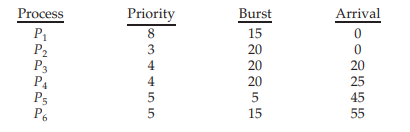
\includegraphics[width=120mm]{a1.png}
        \end{center}\end{figure}
    Each process is assigned a numerical priority, with a higher number indicating a higher relative priority. The scheduler will execute the highest priority process. For processes with the same priority, a round-robin scheduler will be used with a time quantum of 10 units. If a process is
    preempted by a higher-priority process, the preempted process is placed at the end of the queue.
    \begin{enumerate}
        \item [a)]
        Show the scheduling order of the processes using a Gantt chart.
       
       \item [b)]
        What is the turnaround time for each process?
       
       \item [c)]
        What is the waiting time for each process?
    \end{enumerate}

    }
  \begin{solution}
  \par{~}
  \begin{figure}[ht]
    \begin{center}
        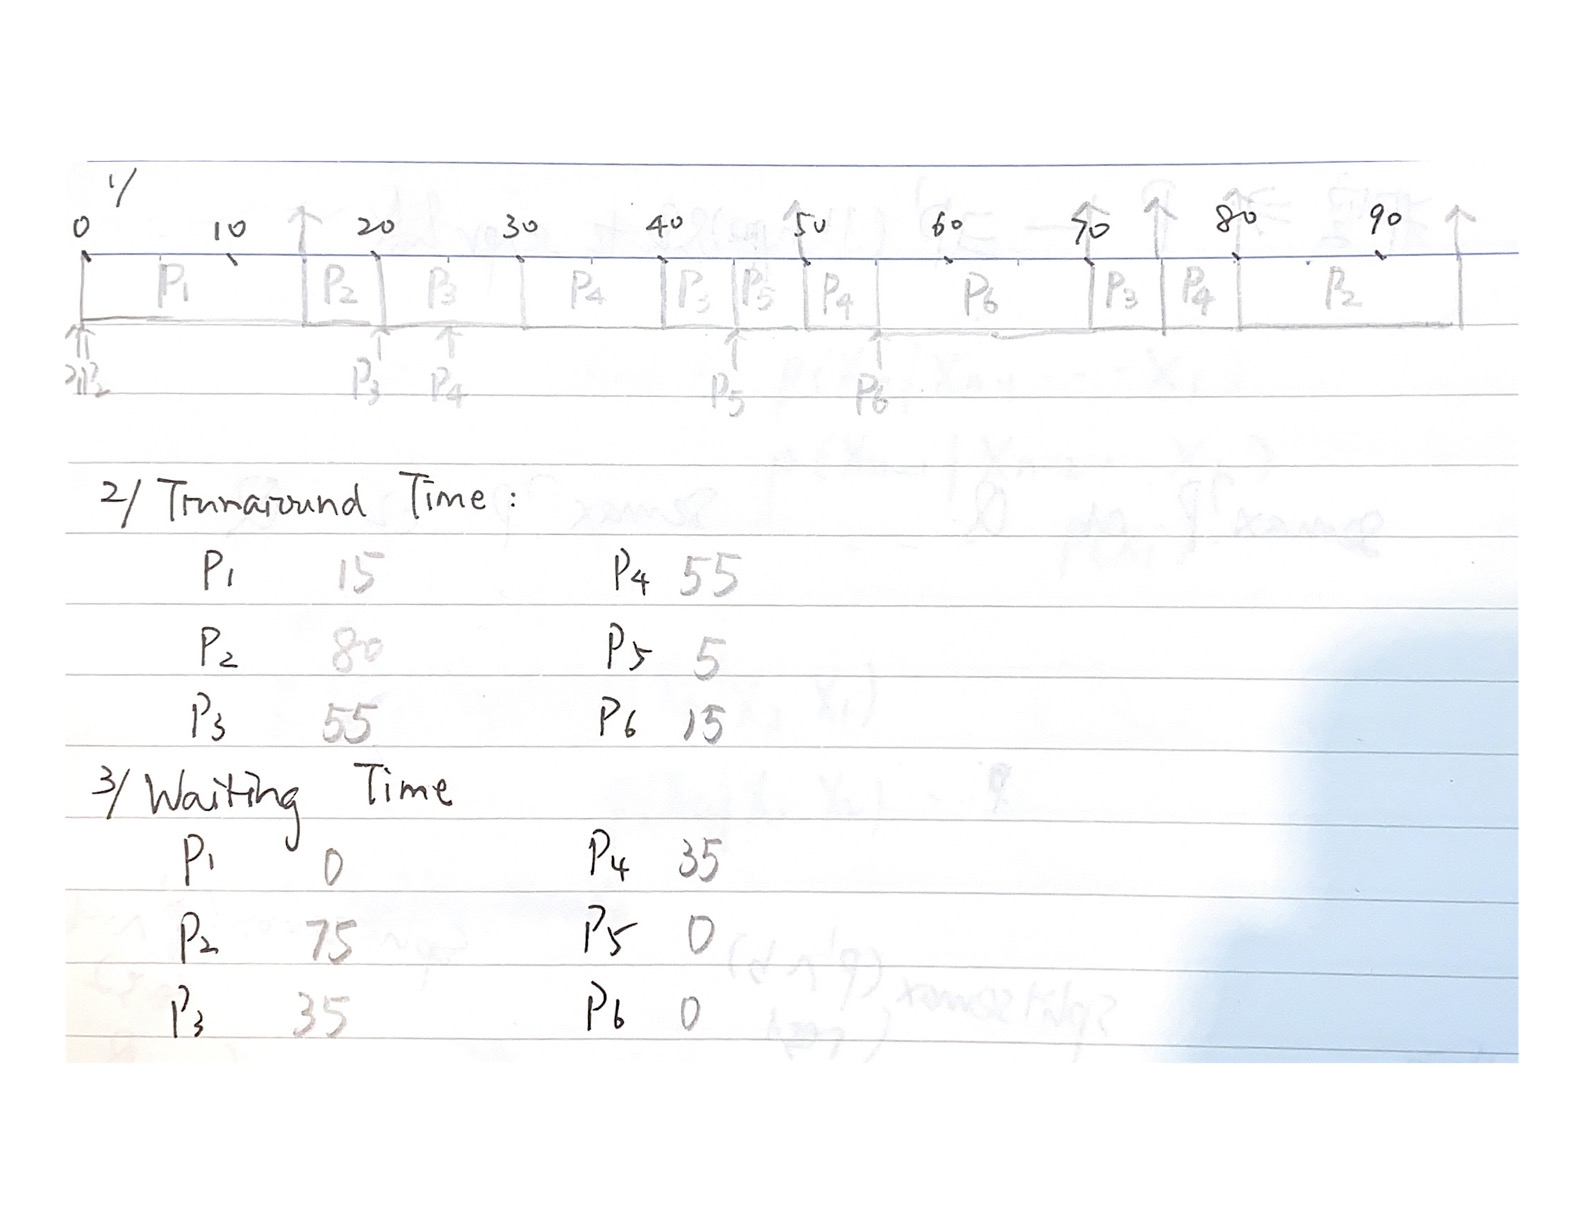
\includegraphics[width=180mm]{ex10.jpg}
    \end{center}\end{figure}
  \end{solution}
  \label{ex1}
\end{exercise}

\newpage
%%%%%%%%%%%%%%%%%%%%%%%%%%%%%%%%%%%%%%%%%%
%%%%%%%%%%%%%                 %%%%%%%%%%%%
%%%%%%%%%%%%%    EXERCISE 2   %%%%%%%%%%%%
%%%%%%%%%%%%%                 %%%%%%%%%%%%
%%%%%%%%%%%%%%%%%%%%%%%%%%%%%%%%%%%%%%%%%%
\begin{exercise}[]{
    Which of the following scheduling algorithms could result in starvation?
    \begin{enumerate}
         \item [a)]
     First-come, first-served
    \item [b)]
    Shortest job first
    \item [c)]
     Round robin
    \item [d)]
     Priority
    \end{enumerate}
}
  \begin{solution}
  \par{~}
  Shortest Job First and Priority may cause starvation. For SJF, processes with extremely long burst may have low priority such that it may never be executed. Similarly, for priority based algorithms, jobs with low priority may never be executed if there are many high priority tasks.
  \end{solution}
  \label{ex2}
\end{exercise}


\end{document}